\documentclass[11pt,a4paper,oneside]{article}
\usepackage[UTF8,adobefonts]{ctex}

\usepackage{wrapfig}
\usepackage{indentfirst}
\usepackage{amsmath}
\usepackage{float}
\usepackage{ulem}

\usepackage[top=1in,bottom=1in,left=1.25in,right=1.25in]{geometry}

\usepackage{color}
\usepackage{xcolor}

\usepackage{multirow}

\begin{document}


\begin{figure}[H]
 \centering
  
\includegraphics[width=13cm]{Image/表头.png}
\end{figure}
\begin{center}
\textbf{{\large 实验名称:\uline{         稳态法测量不良导体的热导率实验      }}}
\end{center}

\section*{一、实验目的}
\begin{enumerate}
\item 熟悉热学实验中的基本问题————量热和计温;
\item 了解热学实验中合理安排实验和选择参量的重要性;
\item 熟悉热学实验中基本仪器的使用。
\end{enumerate}

\section*{二、实验原理}
所谓稳态法,就是设法利用热源在待测样品内部形成不随时间改变的稳定温度分布,然后进行测量。

傅里叶导热方程式指出,在物体内部,取两个垂直于热传导方向、彼此相距为$h$、温度分别为$\Theta _1$、$\Theta _2$ 的平行平面(设$\Theta _1$>$\Theta _2$),若平面面积均为$S$,则在$\delta t$时间内通过面积$S$的热量$\delta Q$满足下述表达式:
$$ \displaystyle\frac{\delta Q}{\delta t}=kS\displaystyle\frac{\Theta _1-\Theta _2}{h} $$
式中,$ \displaystyle\frac{\delta Q}{\delta t}$为热流强度,$k$称为该物质的热导率(又称导热系数)。数值上$k$等于相距单位长度的两平面的温度相差1个单位时,在单位时间内通过单位面积的热量,其单位为$ W/(m\cdot K)$。

\begin{wrapfigure}{r}{0.4\textwidth}
  \vspace{-20pt}
  \begin{center}
    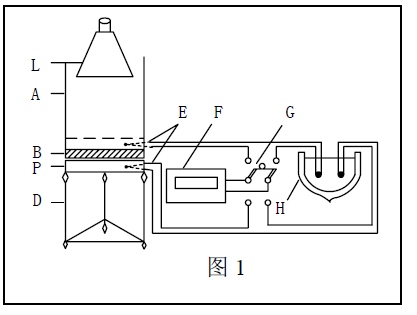
\includegraphics[width=0.48\textwidth]{实验装置.png}
  \end{center}
  \vspace{-20pt}
  \vspace{-10pt}
\end{wrapfigure}

实验装置如图所示,在支架$D$上先后放上圆铜盘$P$、待测样品$B$(圆盘形不良导体)和厚底紫铜圆盘$A$。在$A$的上方用红外灯L加热,使样品上、下表面分别维持在稳定的温度$\Theta _1$、$\Theta _2$,$\Theta _1$、$\Theta _2$分别用插入在$A$、$P$侧面深孔中的热电偶$E$来测量。$E$的冷端浸入盛于杜瓦瓶$H$内的冰水混合物中。$G$为双刀双掷开关,用以换接上、下热电偶的测量回路。实验装置表F用来测量温差电动势。单位时间内通过待测样品$B$任一圆截面的热流量为
\begin{center}
$\displaystyle\frac{\delta Q}{\delta t}= \displaystyle\frac{k\pi d_{B}^{2}}{4} {\times} \displaystyle\frac{\Theta _1-\Theta _2}{h_B}$
\end{center}
式中,$d_{B}$ 为圆盘样品的直径,$h_{B}$为样品厚度。当传热达到稳定状态时,$\Theta _1$ 和$\Theta _2$ 的值不变,这时通过$B$盘上表面的热流量与由黄铜盘$P$向周围环境散热的速率相等。因此,可通过黄铜盘$P$在稳定温度$\Theta _2$ 时的散热速率来求出热流量$\displaystyle\frac{\delta Q}{\delta t}$。实验中,在读得稳定时的$\Theta _1$ 和$\Theta _2$ 后,即可将样品$B$盘移去,而使筒A的底面与盘$P$直接接触。当盘$P$的温度上升到高于稳定时的数值$\Theta _2$若干摄氏度后,再将筒$A$移开,让盘$P$自然冷却。观测其温度$\Theta $随时间$t$的变化情况,然后由此求出黄铜盘在$\Theta _2$的冷却速率$\displaystyle\frac{\delta Q}{\delta t}\|_{\Theta =\Theta _2}$,而$m_pc\displaystyle\frac{\delta \Theta }{\delta t}\|_{\Theta =\Theta _2}$($m_p$为黄铜盘$P$的质量、$c$为其比热容)就是黄铜盘在温度为$Theta _2$ 时的散热速率。但须注意,这样求出的$\displaystyle\frac{\delta \Theta }{\delta t}$是黄铜盘的全部表面暴露于空气中的冷却速率,其散热表面积为$\pi {d_{P}}^{2}/2+\pi d_{P}h_{P}$($d_P$ 与$h_P$ 分别为黄铜盘$P$的直径与厚度)。然而,在观测样品稳态传热时,$P$盘的上表面(面积为$\pi {d_{P}}^{2}/4$)是被样品覆盖着的。考虑到物体的冷却速率与它的表面积成正比,则稳态时黄铜盘散热速率的表达式应修正如下:

$$\displaystyle\frac{{\delta}Q}{{\delta}t} ={m_p}c{\displaystyle\frac{{\delta}{\theta}}{{\delta}t}}{\displaystyle\frac{{\pi}{d^2_P/4}+{\pi}{d_P}{h_P}}{{\pi}{d^2_P/2}+{\pi}{d_P}{h_P}}}$$

最终得:

$$k = {m_P}c{\displaystyle\frac{{\delta}{\theta}}{{\delta}t}}{\displaystyle\frac{{\pi}{d^2_P}/4+{\pi}{d_P}{h_P}}{{\pi}{d^2_P}/2+{\pi}{d_P}{h_P}}}$$

\section*{三、实验仪器}
量热器、电子天平、温度计、数字三用表、加温器皿、冰、水桶、停表、干拭布等;稳态法实验装置。

\section*{四、实验步骤}

\subsubsection*{(1)调整测量系统}

1.根据稳态法,必须得到稳定的温度分布,这就要等待较长的时间。为了提高效率,可先将红外灯的电源电压升高到220V,加热约5min后再降至110V。
然后,每隔2${\sim}$5min读一下温度示值,如在10min内,样品上、下表面温度${\Theta}_1$、${\Theta}_2$ 示值都不变,即可认为已达到稳定状态。记录稳定时的${\Theta} _1$、${\Theta}_2$ 值后,移去样品,再加热。当铜盘温度比${\Theta}_2$ 高出10℃左右时,移去圆筒$A$,让黄铜盘$P$自然冷却。每隔$30s$读一次$P$盘的温度示值,最后选取邻近$\Theta _2$的测量数据来求出冷却速率$\displaystyle\frac{\delta Q}{\delta t}\|_{{\Theta} ={\Theta _2}}$。

2.安置圆筒、圆盘时,注意使放置热电偶的插孔与杜瓦瓶、数字毫伏表位于同一侧。热电偶插入小孔时,要抹些硅油,并插到插孔底部,使热电偶测温端与铜盘接触良好。热电偶冷端插在滴有硅油的细玻管内,再将玻管浸入冰水混合物中。

3.样品圆盘B$B$和黄铜盘$P$的几何尺寸,均可用游标卡尺多次测量取平均。铜盘的质量$m$(约$1kg$)可用电子天平称衡。

4.本实验选用铜-康铜热电偶测温度。热电偶测温的原理是:由两种不同导体或半导体 热电偶温度计组成的闭合回路,如果它们的节点分别处于不同的温度$\Theta _0$和$\Theta $,则回路就会有热电动势$\epsilon (\theta ,\theta _0)$。通常取$\theta _0$=0℃,称为冷端;$\theta $置于被测介质,就可以用$\epsilon$来确定介质的温度。在实际使用时,还需要在热电偶回路中引入不同材料的连接导线和显示仪表。可以证明:只要在热电偶回路中接入的中间导体两端温度相同,热电偶总回路的ε就不会发生改变。基于此,本实验对热电偶温度计作了改装,以增加使用寿命。温差电动势用数字电压表测量。对铜 康铜热电偶而言,温差100℃时,其温差电动势约4.2mV,故应配用能读到0.01mV,且量程不小于$10mV$的数字电压表。
由于热电偶冷端温度为0℃,故对一定材料的热电偶而言,当温度变化范围不太大时,其温差电动势${\epsilon}(mV)$与待测温度${\theta}$(℃)的比值是一个常数。由此,在计算时,可直接以电动势值代表温度值。

\end{document}